% answers.tex —— 1957 年·全国卷 · 参考答案与详细解析片段
% 由 tools/generate_projects.py 依来源总账自 1957/1957_数学真题_试题.md + 1957/1957_数学真题_解析正文.md + 1957/1957_数学真题_答案要点.md 生成，勿手改（改源 MD 后重跑）


\gkpart{一、小题}

\begin{answer}
\gksolhead{1}{}

\textbf{题目}：

（甲）化简
\[
\left(2\frac79\right)^{\frac12}+0.1^{-2}+\left(2\frac{10}{27}\right)^{-\frac23}.
\]

\Needspace{4\baselineskip}
\textbf{解析}

\[
\left(2\frac79\right)^{\frac12}+0.1^{-2}+\left(2\frac{10}{27}\right)^{-\frac23}
=\left(\frac{25}{9}\right)^{\frac12}+100+\frac{1}{\left(\frac{64}{27}\right)^{\frac23}}
\]

\[
\left(2\frac79\right)^{\frac12}+0.1^{-2}+\left(2\frac{10}{27}\right)^{-\frac23}
=\frac53+100+\frac9{16}
\]

\[
\left(2\frac79\right)^{\frac12}+0.1^{-2}+\left(2\frac{10}{27}\right)^{-\frac23}
=102\frac{11}{48}
\]

\gkanswer{答案：$102\dfrac{11}{48}$}

\end{answer}
\begin{answer}
\gksolhead{2}{}

\textbf{题目}：

（乙）求适合不等式 $x^2+x<2$ 的实数 $x$ 的范围。

\Needspace{4\baselineskip}
\textbf{解析}

\[
x^2+x<2
\iff (x+2)(x-1)<0.
\]
故 $-2<x<1$.

\gkanswer{答案：$-2<x<1$}

\end{answer}
\begin{answer}
\gksolhead{3}{}

\textbf{题目}：

（丙）求证
\[
\cot22^\circ30'=1+\sqrt2.
\]
（注：$\cot$ 是余切的符号。）

\Needspace{4\baselineskip}
\textbf{解析}

\[
\cot22^\circ30'=\cot\frac{45^\circ}{2}
=\frac{1+\cos45^\circ}{\sin45^\circ}
=\frac{1+\frac1{\sqrt2}}{\frac1{\sqrt2}}
=1+\sqrt2.
\]

\gkanswer{答案：$\cot22^\circ30'=1+\sqrt2$}

\end{answer}
\begin{answer}
\gksolhead{4}{}

\textbf{题目}：

（丁）在四面体 $ABCD$ 中，$AC=BD$，$P$、$Q$、$R$、$S$ 依次为棱 $AB$、$BC$、$CD$、$DA$ 的中点。求证 $PQRS$ 为一菱形。

\Needspace{4\baselineskip}
\textbf{解析}
\nopagebreak[4]
\begin{center}% 1957 年全国卷第 4 题：四面体棱上四个中点。
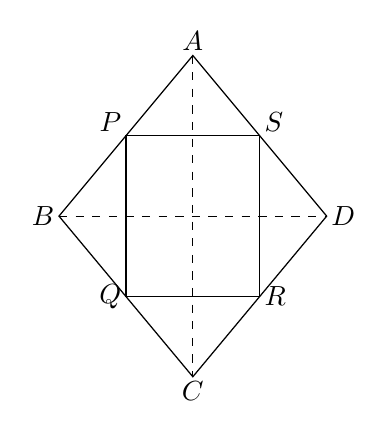
\begin{tikzpicture}[scale=0.85, line width=0.45pt,
  every node/.style={inner sep=1.5pt}]
  \coordinate (A) at (0,2.8);
  \coordinate (B) at (-2,0.4);
  \coordinate (C) at (0,-2.0);
  \coordinate (D) at (2,0.4);
  \coordinate (P) at (-1,1.6);
  \coordinate (Q) at (-1,-0.8);
  \coordinate (R) at (1,-0.8);
  \coordinate (S) at (1,1.6);
  \draw (A)--(B)--(C)--(D)--cycle;
  \draw[dashed] (B)--(D) (A)--(C);
  \draw (P)--(Q)--(R)--(S)--cycle;
  \node[anchor=south] at (A) {$A$};
  \node[anchor=east] at (B) {$B$};
  \node[anchor=north] at (C) {$C$};
  \node[anchor=west] at (D) {$D$};
  \node[anchor=south east] at (P) {$P$};
  \node[anchor=east] at (Q) {$Q$};
  \node[anchor=west] at (R) {$R$};
  \node[anchor=south west] at (S) {$S$};
\end{tikzpicture}
\end{center}
\nopagebreak[4]
由于 $P$、$Q$ 分别为 $AB$、$BC$ 的中点，中点定理给出
\[
PQ\parallel AC,\qquad PQ=\frac12AC.
\]
同理
\[
RS\parallel AC,\qquad RS=\frac12AC.
\]
所以 $PQRS$ 为平行四边形。又因 $R$、$S$ 分别为 $CD$、$DA$ 的中点，
\[
QR=\frac12BD.
\]
由 $AC=BD$，得 $PQ=QR$。平行四边形有一组邻边相等，故 $PQRS$ 为菱形。

\gkanswer{答案：$PQRS$ 为菱形}

\end{answer}
\begin{answer}
\gksolhead{5}{}

\textbf{题目}：

（戊）设 $a$、$b$ 为异面二直线，$EF$ 为 $a$、$b$ 的公垂线，$\alpha$ 为过 $EF$ 中点且与 $a$、$b$ 平行的平面，$M$ 为 $a$ 上任一点，$N$ 为 $b$ 上任一点。求证：线段 $MN$ 被平面 $\alpha$ 二等分。

（注：“异面二直线”也叫“不共面二直线”。）

\Needspace{4\baselineskip}
\textbf{解析}
\nopagebreak[4]
\begin{center}% 1957 年全国卷第 5 题：三平行平面与公垂线中点。
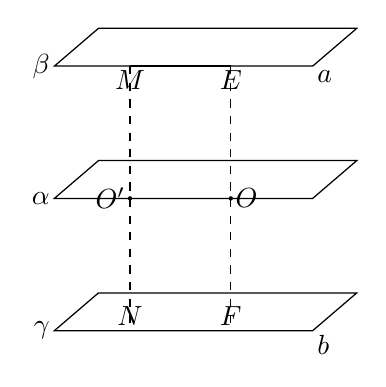
\begin{tikzpicture}[scale=0.8, line width=0.45pt,
  every node/.style={inner sep=1.5pt}]
  \coordinate (A1) at (-2,2.4); \coordinate (B1) at (2.1,2.4);
  \coordinate (C1) at (2.8,3.0); \coordinate (D1) at (-1.3,3.0);
  \coordinate (A2) at (-2,0.3); \coordinate (B2) at (2.1,0.3);
  \coordinate (C2) at (2.8,0.9); \coordinate (D2) at (-1.3,0.9);
  \coordinate (A3) at (-2,-1.8); \coordinate (B3) at (2.1,-1.8);
  \coordinate (C3) at (2.8,-1.2); \coordinate (D3) at (-1.3,-1.2);
  \coordinate (M) at (-0.8,2.4); \coordinate (E) at (0.8,2.4);
  \coordinate (Oprime) at (-0.8,0.3); \coordinate (O) at (0.8,0.3);
  \coordinate (N) at (-0.8,-1.8); \coordinate (F) at (0.8,-1.8);
  \draw (A1)--(B1)--(C1)--(D1)--cycle;
  \draw (A2)--(B2)--(C2)--(D2)--cycle;
  \draw (A3)--(B3)--(C3)--(D3)--cycle;
  \draw[dashed] (M)--(Oprime)--(N) (E)--(O)--(F);
  \draw (M)--(E) (N)--(F);
  \fill (Oprime) circle (0.035) (O) circle (0.035);
  \node[anchor=east] at (A1) {$\beta$};
  \node[anchor=east] at (A2) {$\alpha$};
  \node[anchor=east] at (A3) {$\gamma$};
  \node[anchor=north] at (M) {$M$};
  \node[anchor=north] at (E) {$E$};
  \node[anchor=south] at (N) {$N$};
  \node[anchor=south] at (F) {$F$};
  \node[anchor=east] at (Oprime) {$O'$};
  \node[anchor=west] at (O) {$O$};
  \node[anchor=north west] at (B1) {$a$};
  \node[anchor=north west] at (B3) {$b$};
\end{tikzpicture}
\end{center}
\nopagebreak[4]
设 $O$ 为 $EF$ 的中点，$O'$ 为 $MN$ 与平面 $\alpha$ 的交点。过直线 $a$ 作平面 $\beta\parallel\alpha$，过直线 $b$ 作平面 $\gamma\parallel\alpha$，则
\[
\alpha\parallel\beta\parallel\gamma.
\]
由平行平面截线的比例关系，
\[
MO':O'N=EO:OF.
\]
因 $O$ 是 $EF$ 的中点，$EO=OF$，所以 $MO'=O'N$，即线段 $MN$ 被平面 $\alpha$ 二等分。

\gkanswer{答案：平面 $\alpha$ 将线段 $MN$ 二等分}

\end{answer}
\gkpart{二、大题}

\begin{answer}
\gksolhead{6}{}

\textbf{题目}：

解方程组
\[
\begin{cases}
\lg(2x+1)+\lg(y-2)=1,\\
10^{xy}=10^x\cdot10^y.
\end{cases}
\]
（注：$\lg$ 是以 $10$ 为底的对数 $\log_{10}$ 的符号。）

\Needspace{4\baselineskip}
\textbf{解析}

由对数定义域，必须有
\[
2x+1>0,\qquad y-2>0.
\]
第一式指数化得
\[
(2x+1)(y-2)=10.
\]
第二式由指数函数的单调性得 $xy=x+y$。展开第一式并用 $xy=x+y$ 消元：
\[
2xy-4x+y-12=0,
\]
\[
2(x+y)-4x+y-12=0,
\qquad 2x-3y+12=0.
\]
因此 $y=\dfrac23x+4$。代入 $xy=x+y$，得
\[
2x^2+7x-12=0,
\qquad x=\frac{-7\pm\sqrt{145}}4.
\]
相应
\[
y=\frac23x+4=\frac{17\pm\sqrt{145}}6.
\]
负号分支的 $y=\dfrac{17-\sqrt{145}}6<2$，不满足定义域；正号分支满足 $x>-\dfrac12$、$y>2$。所以唯一解为
\[
x=\frac{-7+\sqrt{145}}4,\qquad y=\frac{17+\sqrt{145}}6.
\]
原卷答案页将 $y$ 的分母误写为 $4$；回代可验证正确分母为 $6$。

\gkanswer{答案：$x=\dfrac{-7+\sqrt{145}}4,\quad y=\dfrac{17+\sqrt{145}}6$}

\end{answer}
\begin{answer}
\gksolhead{7}{}

\textbf{题目}：

若 $\triangle ABC$ 的内切圆半径为 $r$，求证 $BC$ 边上的高 $AD$ 满足
\[
AD=\frac{2r\cos\dfrac B2\cos\dfrac C2}{\sin\dfrac A2}.
\]

\Needspace{4\baselineskip}
\textbf{解析}
\nopagebreak[4]
\begin{center}% 1957 年全国卷第 7 题：三角形内切圆、切点 E 与高 AD。
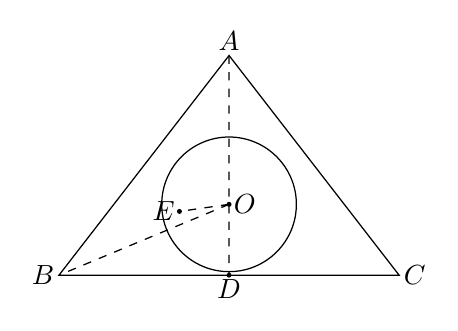
\begin{tikzpicture}[scale=0.9, line width=0.45pt,
  every node/.style={inner sep=1.5pt}]
  \coordinate (B) at (-2.4,0); \coordinate (C) at (2.4,0); \coordinate (A) at (0,3.1);
  \coordinate (D) at (0,0); \coordinate (O) at (0,1.0); \coordinate (E) at (-0.7,0.9);
  \draw (A)--(B)--(C)--cycle;
  \draw (O) circle (0.95);
  \draw[dashed] (A)--(D) (O)--(E) (O)--(B);
  \fill (O) circle (0.035) (D) circle (0.035) (E) circle (0.035);
  \node[anchor=south] at (A) {$A$}; \node[anchor=east] at (B) {$B$};
  \node[anchor=west] at (C) {$C$}; \node[anchor=north] at (D) {$D$};
  \node[anchor=west] at (O) {$O$}; \node[anchor=east] at (E) {$E$};
\end{tikzpicture}
\end{center}
\nopagebreak[4]
设内心为 $O$，内切圆与 $AB$ 的切点为 $E$。则
\[
AE=r\cot\frac A2,\qquad BE=r\cot\frac B2,
\]
从而
\[
AB=r\left(\cot\frac A2+\cot\frac B2\right).
\]
又 $AD$ 是 $BC$ 上的高，故 $AD=AB\sin B$。利用 $A+B+C=180^\circ$，
\[
\cot\frac A2+\cot\frac B2
=\frac{\sin\frac{A+B}{2}}{\sin\frac A2\sin\frac B2}
=\frac{\cos\frac C2}{\sin\frac A2\sin\frac B2}.
\]
再用 $\sin B=2\sin\dfrac B2\cos\dfrac B2$，得
\[
AD=\frac{2r\cos\dfrac B2\cos\dfrac C2}{\sin\dfrac A2}.
\]

\gkanswer{答案：$AD=\dfrac{2r\cos\dfrac B2\cos\dfrac C2}{\sin\dfrac A2}$}

\end{answer}
\begin{answer}
\gksolhead{8}{}

\textbf{题目}：

若 $\triangle ABC$ 为锐角三角形，以 $BC$ 边为直径作圆，并从 $A$ 作此圆的切线 $AD$，与圆切于 $D$，又在 $AB$ 边上取 $AE$ 等于 $AD$，并过 $E$ 作 $AB$ 的垂线与 $AC$ 边的延长线交于 $F$，求证：

（1）$AE:AB=AC:AF$；

（2）$\triangle ABC$ 的面积等于 $\triangle AEF$ 的面积。

\Needspace{4\baselineskip}
\textbf{解析}
\nopagebreak[4]
\begin{center}% 1957 年全国卷第 8 题：以 BC 为直径的圆、切点 D 与辅助点 G。
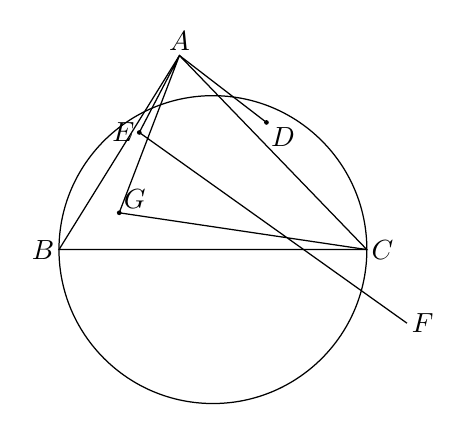
\begin{tikzpicture}[scale=0.85, line width=0.45pt,
  every node/.style={inner sep=1.5pt}]
  \coordinate (B) at (-2.3,0); \coordinate (C) at (2.3,0);
  \coordinate (O) at (0,0); \coordinate (A) at (-0.5,2.9);
  \coordinate (D) at (0.8,1.9); \coordinate (E) at (-1.1,1.75);
  \coordinate (G) at (-1.4,0.55); \coordinate (F) at (2.9,-1.1);
  \draw (O) circle (2.3);
  \draw (A)--(B)--(C)--cycle;
  \draw (A)--(D) (A)--(E)--(F) (A)--(G)--(C);
  \draw (B)--(C);
  \fill (D) circle (0.035) (E) circle (0.035) (G) circle (0.035);
  \node[anchor=south] at (A) {$A$}; \node[anchor=east] at (B) {$B$};
  \node[anchor=west] at (C) {$C$}; \node[anchor=north west] at (D) {$D$};
  \node[anchor=east] at (E) {$E$}; \node[anchor=south west] at (G) {$G$};
  \node[anchor=west] at (F) {$F$};
\end{tikzpicture}
\end{center}
\nopagebreak[4]
设直线 $AB$ 与圆的另一个交点为 $G$。由切割线定理，
\[
AG\cdot AB=AD^2.
\]
由于 $AE=AD$，故
\[
\frac{AG}{AE}=\frac{AE}{AB}.
\]
又因 $BC$ 是圆的直径，$\angle BGC=90^\circ$，所以 $GC\perp AB$。而 $EF\perp AB$，故 $GC\parallel EF$。于是
\[
\frac{AG}{AE}=\frac{AC}{AF},
\]
从而
\[
\frac{AE}{AB}=\frac{AC}{AF}.
\]
这证明了第（1）问。进一步
\[
AB\cdot AC=AE\cdot AF.
\]
两三角形有公共角 $\angle A$，所以
\[
\frac{S_{\triangle ABC}}{S_{\triangle AEF}}
=\frac{AB\cdot AC}{AE\cdot AF}=1,
\]
即 $S_{\triangle ABC}=S_{\triangle AEF}$。

\gkanswer{答案：$AE:AB=AC:AF$，且 $S_{\triangle ABC}=S_{\triangle AEF}$}

\end{answer}
\begin{answer}
\gksolhead{9}{}

\textbf{题目}：

求证：方程
\[
x^3-(\sqrt2+1)x^2+(\sqrt2-q)x+q=0
\]
的一个根是 $1$。设这个方程的三个根是一个 $\triangle ABC$ 的三个内角的正弦 $\sin A$、$\sin B$、$\sin C$，求 $A$、$B$、$C$ 的度数及 $q$ 的数值。

\Needspace{4\baselineskip}
\textbf{解析}

将 $x=1$ 代入原方程，得
\[
1-(\sqrt2+1)+(\sqrt2-q)+q=0,
\]
所以 $1$ 确为方程的根。因式分解得
\[
x^3-(\sqrt2+1)x^2+(\sqrt2-q)x+q
=(x-1)(x^2-\sqrt2x-q).
\]
三个根是 $\sin A$、$\sin B$、$\sin C$，其中必有一个等于 $1$。不妨设 $\sin C=1$，则 $C=90^\circ$，$A+B=90^\circ$。

另外两个根满足
\[
\sin A+\sin B=\sqrt2,
\qquad \sin^2A+\sin^2B=1.
\]
因此
\[
2\sin A\sin B=2-1=1,
\qquad (\sin A-\sin B)^2=0.
\]
故 $A=B=45^\circ$。由二次因式根的乘积，
\[
-q=\sin A\sin B=\frac12,
\qquad q=-\frac12.
\]

\gkanswer{答案：$A$、$B$、$C$ 为 $45^\circ$、$45^\circ$、$90^\circ$（角的排列可互换），$q=-\dfrac12$}

\end{answer}